% !Tex Program = xelatex
% -*-coding: utf-8 -*-
\documentclass[12pt,onecolumn]{report}

% 中文
\usepackage[BoldFont,SlantFont]{xeCJK}
\xeCJKsetemboldenfactor{1}%只对随后定义的CJK字体有效
\setCJKfamilyfont{hei}{SimHei}
\xeCJKsetemboldenfactor{4}
\setCJKfamilyfont{song}{SimSun}
\xeCJKsetemboldenfactor{4}
\setCJKfamilyfont{fs}{FangSong}
\setCJKfamilyfont{kai}{KaiTi}
\setCJKfamilyfont{li}{LiSu}
\setCJKfamilyfont{xw}{STXinwei}
\setCJKmainfont[BoldFont=SimHei]{SimSun}
\setCJKmonofont{SimSun}
\setCJKsansfont{SimSun}

\newcommand{\hei}{\CJKfamily{hei}}      % 黑体
\newcommand{\song}{\CJKfamily{song}}    % 宋体   (Windows 自带simsun.ttf)
\newcommand{\fs}{\CJKfamily{fs}}        % 仿宋体 (Windows 自带simfs.ttf)
\newcommand{\kai}{\CJKfamily{kai}}      % 楷体   (Windows 自带simkai.ttf)
\newcommand{\li}{\CJKfamily{li}}        % 隶书   (Windows自带simli.ttf)
\newcommand{\xw}{\CJKfamily{xw}}        % 隶书   (Windows自带simli.ttf)

% \AmSTeX\ 宏包,用来排出更加漂亮的公式。
\usepackage{amsmath}
% 定理类环境宏包,其中 \pkg{amsmath} 选项用来兼容 \AmSTeX\ 的宏包
\usepackage[amsmath,thmmarks,hyperref]{ntheorem}
\usepackage{amssymb}
% 添加字体
\usepackage[defaultsups]{newtxtext}
\usepackage{newtxmath}
\usepackage{courier}
% 图形支持宏包
\usepackage{graphicx}
% 插入pdf
\usepackage{pdfpages}
\includepdfset{fitpaper=true}
% 更好的列表环境。
\usepackage{enumitem}       %使用enumitem宏包,改变列表项的格式
\usepackage{environ}
% 禁止 \LaTeX 自动调整多余的页面底部空白,并保持脚注仍然在底部。
% 脚注按页编号。
\usepackage[bottom,perpage,hang]{footmisc}
\raggedbottom{}
% 脚注格式。
\usepackage{pifont}
% 表格控制
\usepackage{longtable}
\usepackage{booktabs}
% 参考文献引用宏包
\usepackage[sort&compress,numbers]{natbib}
% 生成有书签的 pdf 及其开关,请结合 gbk2uni 避免书签乱码。
\usepackage{hyperref}
\hypersetup{
  CJKbookmarks=true,
  linktoc=all,
  bookmarksnumbered=true,
  bookmarksopen=true,
  bookmarksopenlevel=1,
  breaklinks=true,
  colorlinks=false,
  plainpages=false,
  pdfborder=0 0 0}
% 设置 url 样式,与上下文一致
\urlstyle{same}
% 版芯设置
\usepackage{geometry}
\geometry{
  a4paper,
  centering,
  text={150true mm,236true mm},
  left=30true mm,
  head=5true mm,
  headsep=2true mm,
  footskip=0true mm,
  foot=5.2true mm
}
% 利用 \pkg{fancyhdr} 设置页眉页脚。
\usepackage{fancyhdr}
% 其他包,表格、数学符号包
\usepackage{tabularx}
\usepackage{varwidth}
% 此处changepage环境用来控制索引页面的左右边距,规范中给出的示例的边距要大于正文。
\usepackage{changepage}
% 多栏结构在文中用begin{multicols}{2}end{multicols}
\usepackage{multicol,multienum}
% 允许上一个section的浮动图形出现在下一个section的开始部分,还提供\FloatBarrier命
% 令,使所有未处理的浮动图形立即被处理
\usepackage[below]{placeins}
% 支持子图 %centerlast 设置最后一行是否居中
\usepackage{subfigure}
% 支持双语标题
\usepackage[subfigure]{ccaption}
% 根据我工规定,正文小四号 (12bp) 字,行距为固定值3--4mm。
\renewcommand\normalsize{
  \abovedisplayskip=8pt
  \abovedisplayshortskip=8pt
  \belowdisplayskip=\abovedisplayskip{}
  \belowdisplayshortskip=\abovedisplayshortskip}
% 根据习惯定义字号。用法:\cs{hit@def@fontsize}\marg{字号名称}\marg{磅数}避免了
% 字号选择和行距的紧耦合。所有字号定义时为单倍行距,并提供选项指定行距倍数。
\def\hit@def@fontsize#1#2{%
  \expandafter\newcommand\csname #1\endcsname[1][1.3]{%
    \fontsize{#2}{##1\dimexpr #2}\selectfont}}
\hit@def@fontsize{dachu}{58bp}
\hit@def@fontsize{chuhao}{42bp}
\hit@def@fontsize{xiaochu}{36bp}
\hit@def@fontsize{yihao}{26bp}
\hit@def@fontsize{xiaoyi}{24bp}
\hit@def@fontsize{erhao}{22bp}
\hit@def@fontsize{xiaoer}{18bp}
\hit@def@fontsize{sanhao}{16bp}
\hit@def@fontsize{xiaosan}{15bp}
\hit@def@fontsize{sihao}{14bp}
\hit@def@fontsize{banxiaosi}{13bp}
\hit@def@fontsize{xiaosi}{12bp}
\hit@def@fontsize{dawu}{11bp}
\hit@def@fontsize{wuhao}{10.5bp}
\hit@def@fontsize{xiaowu}{9bp}
\hit@def@fontsize{liuhao}{7.5bp}
\hit@def@fontsize{xiaoliu}{6.5bp}
\hit@def@fontsize{qihao}{5.5bp}
\hit@def@fontsize{bahao}{5bp}
% 利用 \pkg{enumitem} 命令调整默认列表环境间的距离,以符合中文习惯。
\setlist{nosep}
% 允许太长的公式断行、分页等。
\allowdisplaybreaks[4]
\predisplaypenalty=0  %公式之前可以换页,公式出现在页面顶部
\postdisplaypenalty=0
% 公式编号设置
\renewcommand{\theequation}{\arabic{chapter}.\arabic{equation}}
% 定理标题使用黑体,正文使用宋体,冒号隔开。
\theorembodyfont{\normalfont}
\theoremheaderfont{\normalfont\hei}
\theoremsymbol{\ensuremath{\square}}
\newtheorem*{proof}{证明}
\theoremstyle{plain}
\theoremsymbol{}
\theoremseparator{}
\newtheorem{assumption}{假设}[chapter]
\newtheorem{definition}{定义}[chapter]
\newtheorem{proposition}{命题}[chapter]
\newtheorem{lemma}{引理}[chapter]
\newtheorem{theorem}{定理}[chapter]
\newtheorem{axiom}{公理}[chapter]
\newtheorem{corollary}{推论}[chapter]
\newtheorem{exercise}{练习}[chapter]
\newtheorem{example}{例}[chapter]
\newtheorem{remark}{注释}[chapter]
\newtheorem{problem}{问题}[chapter]
\newtheorem{conjecture}{猜想}[chapter]
% 各种单位
\usepackage{siunitx}
\sisetup{group-minimum-digits=4, group-separator= \hspace{0.25em}}
\sisetup{detect-weight,detect-mode,detect-family}
% 处理数学公式中的黑斜体的宏包
\usepackage{bm}
% 不同于 \mathcal \mathfrak 之类的英文花体字体
\usepackage{mathrsfs}
% 支持彩色
\usepackage[table]{xcolor}
\definecolor{colorzero}{rgb}{0, 0, 0}
\definecolor{colorone}{rgb}{1, 0, 0}
\definecolor{colortwo}{rgb}{0, 0, 1}
\definecolor{colorthree}{rgb}{0, 1, 0}
% 图形和表格的控制旋转
\usepackage{rotating}
% 算法的宏包,注意宏包兼容性,先后顺序为float、hyperref、algorithm(2e),否则无法
% 生成算法列表。
\usepackage[algoruled,linesnumbered]{algorithm2e}
% 排版源码所使用的环境。
\usepackage{listings}
\lstset{
  language    = c++,
  breaklines  = true,
  frame       = single,
  captionpos  = b,
  tabsize     = 2,
  numbers     = left,
  columns     = fixed,
  keepspaces  = true,
  commentstyle = \slshape\color[RGB]{0,96,96},
  keywordstyle = \color[RGB]{40,40,255},
  basicstyle   = \ttfamily,
  rulesepcolor = \color{red!20!green!20!blue!20},
  numberstyle  = \color{darkgray},
  stringstyle  = \color[RGB]{128,0,0},
  % backgroundcolor = \color[RGB]{245,245,244},
  showstringspaces = false,
  morekeywords={alignas,continute,friend,register,true,alignof,decltype,goto,
    reinterpret_cast,try,asm,defult,if,return,typedef,auto,delete,inline,short,
    typeid,bool,do,int,signed,typename,break,double,long,sizeof,union,case,
    dynamic_cast,mutable,static,unsigned,catch,else,namespace,static_assert,using,
    char,enum,new,static_cast,virtual,char16_t,char32_t,explict,noexcept,struct,
    void,export,nullptr,switch,volatile,class,extern,operator,template,wchar_t,
    const,false,private,this,while,constexpr,float,protected,thread_local,
    const_cast,for,public,throw,std},
  emph={map,set,multimap,multiset,unordered_map,unordered_set,
    unordered_multiset,unordered_multimap,vector,string,list,deque,
    array,stack,forwared_list,iostream,memory,shared_ptr,unique_ptr,
    random,bitset,ostream,istream,cout,cin,endl,move,default_random_engine,
    uniform_int_distribution,iterator,algorithm,functional,bing,numeric,},
  emphstyle=\color{CPPViolet},
}

% 作图
\usepackage{tikz}
\usetikzlibrary{graphs, positioning, quotes, shapes.geometric}

% 首行缩进
\usepackage{indentfirst}
\setlength{\parindent}{2em}

\usepackage{float}
\usepackage{diagbox}
\usepackage{setspace}
\usepackage{zhnumber}
\usepackage{titlesec}

% \renewcommand\thechapter{\zhnum{chapter}}
% \renewcommand\thesection{\arabic{section}}

\titleformat{\chapter}{\centering\Huge\bfseries}{第\,\thechapter\,章}{1em}{}
% \titleformat{\section}{\raggedright\Large\bfseries}{\thesection\,}{1em}{}
% \titleformat{\subsection}{\raggedright\large\bfseries}{\,\thesubsection\,}{1em}{}
% \titleformat{\subsubsection}{\raggedright\large\bfseries}{\,\thesubsubsection\,}{1em}{}

\graphicspath{{figures/}}
\bibliographystyle{plainnat}

\pagestyle{fancy}
\fancyhead[L]{\song\xiaowu[0]{1180100217~郭炼}}
\fancyhead[C]{\song\xiaowu[0]{数据库实验二报告}}
\fancyhead[R]{\song\xiaowu[0]{哈尔滨工业大学}}
\fancyfoot[C]{\xiaowu-~\thepage~-}
\makeatletter
\def\headrule{{%
    \if@fancyplain\let\headrulewidth\plainheadrulewidth\fi
    \vskip2pt
    \hrule\@height2pt\@width\headwidth\vskip1pt
    \hrule\@height\headrulewidth\@width\headwidth\vskip-\headrulewidth\vskip-4pt
  }}
\makeatother

\fancypagestyle{plain}{
  \fancyhf{}
  \fancyhead[L]{\song\xiaowu[0]{1180100217~郭炼}}
  \fancyhead[C]{\song\xiaowu[0]{数据库实验二报告}}
  \fancyhead[R]{\song\xiaowu[0]{哈尔滨工业大学}}
  \fancyfoot[C]{\xiaowu-~\thepage~-}
}

\renewcommand{\today}{\number\year{年}\number\month{月}\number\day{日}}
\renewcommand{\contentsname}{\centering \hei{目录}}
\renewcommand{\figurename}{图}
\renewcommand{\tablename}{表}
\renewcommand{\lstlistingname}{代码}
\numberwithin{figure}{chapter}
\numberwithin{table}{chapter}
\numberwithin{lstlisting}{chapter}

\renewcommand{\baselinestretch}{1.25}
\newcommand{\M}[1]{\mathbf{#1}}
\setcounter{secnumdepth}{4}

\begin{document}

\begin{titlepage}
  \vspace{5\baselineskip}

  \begin{figure}[H]
    \centering
    
\includegraphics[width=0.6\linewidth]{figures/school.eps}
  \end{figure}

  \centering\hei{}

  \xiaosan\vspace{\baselineskip}

  \makebox[150bp][s]{数据库实验二报告}

  \erhao\vspace{2\baselineskip}

  \makebox[400bp][s]{实验二:缓冲池管理器(Buffer Manager)}

  \sanhao\vspace{3\baselineskip}

  \makebox[80bp][s]{姓名}~~\underline{\makebox[160bp][s]{郭炼}} \\ [24pt]
  \makebox[80bp][s]{学号}~~\underline{\makebox[160bp][s]{1 1 8 0 1 0 0 2 1 7}} \\ [24pt]
  \makebox[80bp][s]{老师}~~\underline{\makebox[160bp][s]{邹兆年}} \\ [24pt]
  \makebox[80bp][s]{专业}~~\underline{\makebox[160bp][s]{数据科学与大数据技术}} \\ [24pt]
  \makebox[80bp][s]{日期}~~\underline{\makebox[160bp][s]{2020 年 05 月 25 日}} \\ [24pt]
\end{titlepage}

\clearpage
\tableofcontents
\clearpage

\makeatletter
\patchcmd{\chapter}{\if@openright\cleardoublepage\else\clearpage\fi}{}{}{}
\makeatother

\chapter{实验目的}
在本次实验中,
我需要基于 BadgerDB 已经实现的存储管理器,
采用时钟算法作为缓冲池替换策略管理缓冲页,
实现 BadgerDB 缓冲池管理器。

\chapter{缓冲池替换策略}
\section{时钟算法}
在本次实验中,我们使用
时钟算法作为缓冲池替换策略管理缓冲页。

我们将缓冲池的所有页看成一个环,
维护一个时钟指针来指示当前的页。
每次申请新页时,我们首先移动时钟指针,
之后查看当前页是否空闲:
如果为空,就直接返回当前空页;
如果不为空,就查看是否空闲。
如果空闲就写回缓冲(如果必要)再返回。
如果所有页都被占用着,就抛出一个异常。
该算法对应的流程图如图\ref{fig:clock}所示。

\begin{figure}[ht]
  \centering
  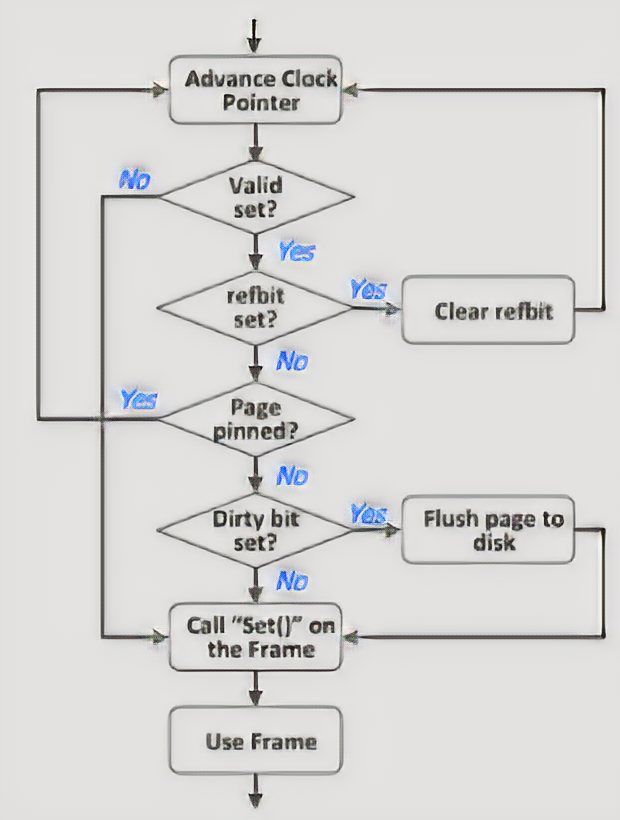
\includegraphics{figures/clock.png}
  \caption{时钟算法流程图\label{fig:clock}}
\end{figure}

\chapter{代码实现}
我们只需要编辑 buffer.cpp 文件,
实现 \lstinline|Buffer| 类对应的方法就可以完成本次实验。

\section{析构算法}
在析构函数中,我们只需要做两件事:
写回脏页和释放内存。
程序会将所有合法的有效脏页写回到磁盘,
之后将占用的所有堆内存释放(如 hashTable,bufPool 等)到堆上。

\section{advanceClock 方法}
在 \lstinline|advanceClock| 方法我们只需要让时钟指针前进一步就可以了。

需要注意的是,由于缓冲页逻辑上是环形的,
所以如果指针到达终点后面(\lstinline|clockHand == numBufs|),我们需要将指针移回至起点。

\section{allocBuf 方法}
\lstinline|allocBuf| 方法需要
返回一个空闲的页用于其他程序来使用。
在该方法中,我们需要实现时钟算法(参见第二章),同时更新哈希表。

如果程序找到一个可用的页,那么就会设置参数中的 frame 来返回;
否则就抛出 \lstinline|BufferExceededException| 异常。

\section{readPage 方法}
\lstinline|readPage| 方法则是用于读取特定页。
其参数为\lstinline|File* file, const PageId PageNo, Page*& page|,
其中 \lstinline|file, PageNo| 用于定义查询对应的页。
\lstinline|page| 则用于返回对应页指针。

程序会首先在哈希表中查询对应的页。
如果找到,则表明该页已经在缓冲池中,
那么只需要更新描述表中 \lstinline|refbit, pinCnt|
两个变量即可,之后返回该页;
如果没有找到,那么表明我们需要使用 \lstinline|allocBuf| 方法
来为该页申请一个新的缓冲池,
之后更新描述表,在哈希表中插入对应项。

\section{unPinPage 方法}
\lstinline|unPinPage| 方法用于释放一个页的占用。
具体来说就是将在哈希表中差点对应的缓冲,
将其对应描述表的 \lstinline|pinCnt| 减一。
如果此时 \lstinline|pinCnt| 为零,
则抛出 \lstinline|PageNotPinnedException| 异常。

如果该页不在哈希表中,
则表明该页在缓冲池中没有对应的缓冲块,
那么就不需要更新任何数据。

\section{allocPage 方法}
\lstinline|allocPage| 方法用于将给定文件的页读入缓冲池中。
我们可以使用 \lstinline|file| 的 \lstinline|allocatePage| 方法
来在对应的文件中申请一个新的空页,
之后利用 \lstinline|allocBuf| 方法来申请新的缓冲块,
将申请的新页与新的缓冲块建立其联系,
并在哈希表中插入对应的项,同时更新描述表。

在完成这一切之后,更新 \lstinline|PageNo, page|
两个变量来传出新页和缓冲块的数据。

\section{disposePage 方法}
\lstinline|disposePage| 方法用于将指定页从文件中删除。
如果该页在缓冲池中有对应的块,
那么同时也需要同步清空对应的描述表,删除哈希表中对应项,释放该块。

\section{flushFile 方法}
\lstinline|flushFile| 方法将给定文件的全部缓冲页全部写回,
并在哈希表中删除对应的项,清空描述表中对应信息。
需要注意的是:
\begin{itemize}[fullwidth,itemindent=\parindent]
\item
  若删除的块无效,则需要抛出 \lstinline|BadBufferException| 异常;
\item
  若该块正在被其他程序占用,则需要抛出 \lstinline|PagePinnedException| 异常。
\end{itemize}

\chapter{实验总结}
在本次实验中,
我对于缓冲池管理器的工作机制有了更为清晰和具体的理解,
学习到数据库中缓冲池的工程细节和原理,
对于缓冲池的页管理有更深入的理解,
同时提升了 C++ 的工程代码能力。

在对自己的代码调试的过程中,
我也感受到了数据库系统的复杂性和综合性。
数据库缓冲池涉及了许多对于内存和文件的操作,
而一旦操作失误,如果没有足够的检查,报错不够及时,
那么就会在出现错误时无从查起,需要溯源多级。

\end{document}
